% !TEX root = ../HDR.tex
%%%%%%%%%%%%%%%%%%%%%%%%%%%%%%%%%%%%%%%%%%%%%%%%%%%%%%%%%%%%%%%%%%%%%%%%%%%%%%%%%%
\chapter{Etat de l'art}

Ce chapitre passe en revue l'état de l'art dans le domaine de l'intelligence artififielle, l'apprentissage artificiel, et l'informatique qui est pertinent pour le problème de l'intelligence artificielle développementale. 

La première partie porte sur l'apprentissage autonome artificiel et vise à pauser les concepts de base de ce problème. 
La seconde partie passe en revue certaines approches techniques de façon à présenter le formalisme mathématique utilisé dans la littérature, sur lequel nous pourrons nous appuyer dans les chapitres suivants. 



\section{Apprentissage autonome}

Définir l'autonomie des agents artificiels n'est pas aussi facile qu'il n'y parait. 
David Vernon \cite{vernon_artificial_2014} identifie plusieurs types d'autonomie


\subsection{Système de décision discret}

\noindent
La façon la plus générale de modéliser un système d'IA repose sur le modèle \an{Discret Decision System} (DDS) illustré en Fig. \ref{fig:dds}.
Dans ce modèle, on peut désigner le système d'IA par le terme \an{software} qui englobe les notions de programme, de logiciel, ou d'algorithme au sens large. 
Ce \an{software} échange des informations au cours d'un \textit{cycle d'interaction discret} qui alterne les \emph{entrées} reçues de son environnement et les \emph{sorties} émises vers son environnement. 

\begin{figure}[h]
	\centering
	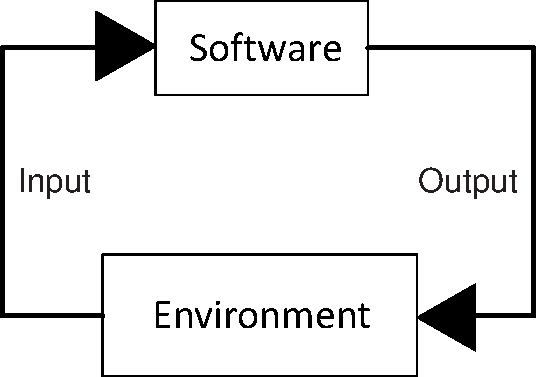
\includegraphics[width=0.3\textwidth]{Figures/1_dds.pdf}
	\caption{Système de décision discret (DDS). Au cours de chaque cycle d'interaction, le \an{software} reçoit un \an{input} en provenance de son environnement et émet un \an{output} en direction de son environnement.
	}
	\label{fig:dds}
\end{figure}

Le DDS est si général qu'il s'applique à l'ensemble des domaines de l'IA, depuis la robotique jusqu'aux agents conversationnels. 
En robotique, l'\an{input} correspond à l'état des \emph{registres d'entrée} déterminés par les capteurs, et l'\an{output} désigne l'état des \emph{registres de sortie} qui commandent les actionneurs. 
Dans ce cas, la durée du cycle d'interaction s'exprime parfois en millisecondes. 
Dans le cas d'un agent conversationnel, l'\an{input} est le \an{prompt} de l'utilisateur, et l'\an{output} la réponse du modèle de langage. 
La durée du cycle d'interaction peut alors s'exprimer en minutes. 

Le \an{software} peut être un algorithme univoque qui produit toujours la même sortie pour une entrée donnée, ou il peut contenir une mémoire qui modifie le traitement au cours du temps.
Il peut aussi contenir un mécanisme stochatistique qui inclut une composante aléatoire dans la génération de la sortie. 
Par exemple, la plupart des grands modèles de langages sont \emph{univoques stochastiques} au sens ou un \an{prompt} donné conserve la même probabilité de produire une réponse donnée. 

Le modèle DDS puise ses origines dans la cybernétique et la théorie des automates à états finis.
%Bien qu'il ne soit pas attribué à un autour particulier, on en retrouve différentes formulations dans la littérature en intelligence artificielle et en apprentissage machine. 
Ben Goertzel y fait explicitement référence dans sa \an{General Theory of General Intelligence} \cite{goertzel_general_2021}. 
L'ouvrage de référence \textit{Artificial Intelligence, a modern approach} de Stuart Russell et Peter Norvig, de son coté, y fait implicitement référence en annonçant que  \og \an{the problem of AI is to build agents that receive percepts from the environment and perform actions} \fg\   \cite[p.~iv]{russell_artificial_2021}.
%en faisant référence au modèle similaire de \an{Marvok Decision Process} (MDP) \cite[p.~iv]{russell_artificial_2021}, que je présenterai dans en Section \ref{sec:rl} consacrée à l'apprentissage par renforcement.
%A ma connaissance, la littérature n'offre pas d'alternative significative à ce découpage en pas de temps discrets. 
Ce découpage en pas de temps discrets trouve aussi une justification bio-inspirée dans le constat que le cerveau est cadencé par des vagues de déclenchement synaptiques périodiques à la fréquence des ondes gamma.

%Tout d'abord, le terme \textit{action} n'est peut-être pas le plus adéquat pour désigner l'information transmise de l'agent vers l'environnement.

Sans remettre en cause le modèle DDS, il convient de garder à l'esprit certaines de ses limites.
Une première limite tient au fait qu'il tend à prendre pour acquis qu'on puisse assimiler l'\an{output} du \an{software} à l'action de agent.  
Dans leur article \og \an{Where's the action? The pragmatic turn in cognitive science} \fg, Andreas Engel et ses coauteurs critiquent cette assimulation entre \an{output} et action. %en s'appuyant sur la définition donnée par la \an{Stanford Encyclopedia of Philosophy}.
Selon eux, une \an{action} n'est pas un simple signal de sortie mais un contrôle intentionnel de l'environnement en vu d'une certaine finalité anticipée :
\begin{quote}
	\an{actions (i) are driven by goals and [...] they can reach these goals or fail to do so; (ii) often involve some degree of volitional control; (iii) require planning and decisions among alternatives; (iv) involve prediction or anticipation of an intended outcome; (v) are often, albeit not always, associated with a sense of agency, that is, the agent’s conscious awareness of carrying out the particular action and of its goals}
	\cite[p.~202]{engel_wheres_2013}.
\end{quote}

\noindent
Engel nous incite à garder à l'esprit que l'\an{output} ne représente pas nécessairement une action au sens intentionnel du terme. 


Une seconde limite du DDS est qu'il présuppose une séparation nette entre l'agent et l'environnement. 
L'agent est défini avec des contours bien établis qui le distinguent de son environnement, et les types d'interactions possibles sont prédéfinies par le concepteur. 
Ce modèle écarte donc la question du processus d'émergence de la frontière entre l'agent et l'environnement, qui est un des aspects du processus d'\emph{individuation} de l'agent que j'ai évoqué en Section \ref{sec:individuation}.
David Weinbaum et Viktoras Veitas notent que cette émergence pourrait impliquer une forme d'intelligence qui n'est pas prise en compte par le DDS. 
Dans leur article \og \an{Open ended intelligence: The individuation of intelligent agents} \fg, ils critiquent une définition de l'intelligence qui présuppose la distinction entre l'agent et l'environnement : 

\begin{quote}
	\an{Processes of differentiation and boundary formation that determine the agent-environment distinctions are excluded. Such processes that can be broadly categorized as processes of self-organization can be gradual and possibly express intelligence of a kind that is not considered by this definition}
	\cite[p.~5]{weinbaum_open_2015}.
\end{quote}

Une troisième critique porte sur la séparation stricte entre \an{input} et \an{output} qui tend à minimiser l'importance de leur couplage réciproque et de leur interdépendance. 
Il est fréquent que les données d'entrée de l'agent n'aient de sens qu'en relation avec l'action qui les a précédées. 
Par example, dans la cybernétique de Norbert Wiener \cite{wiener_cybernetics_1948}, les données d'entrée constituent des \emph{rétroactions} (\an{feedback}) résultant de l'action.  
De plus, les actions peuvent aussi posséder une structure hiérarchique : certaines actions de haut niveau se découpant en séries d'actions de plus bas niveau.
Différentes actions peuvent parfois être exécutées en parallèle au cours de périodes de temps qui se recouvrent.
Si le modèle DDS n'exclut pas de telles possibilités, il comporte néanmoins le risque de conduire à une vision trop appauvrie des systèmes d'IA.
Pour illustrer cette diversité de situations, la Figure \ref{fig:dds2} propose différentes déclinaisons du DDS, en remplaçant les termes \an{input} et \an{output} par des termes plus spécialisés. 


\begin{figure}[h]
	\centering
	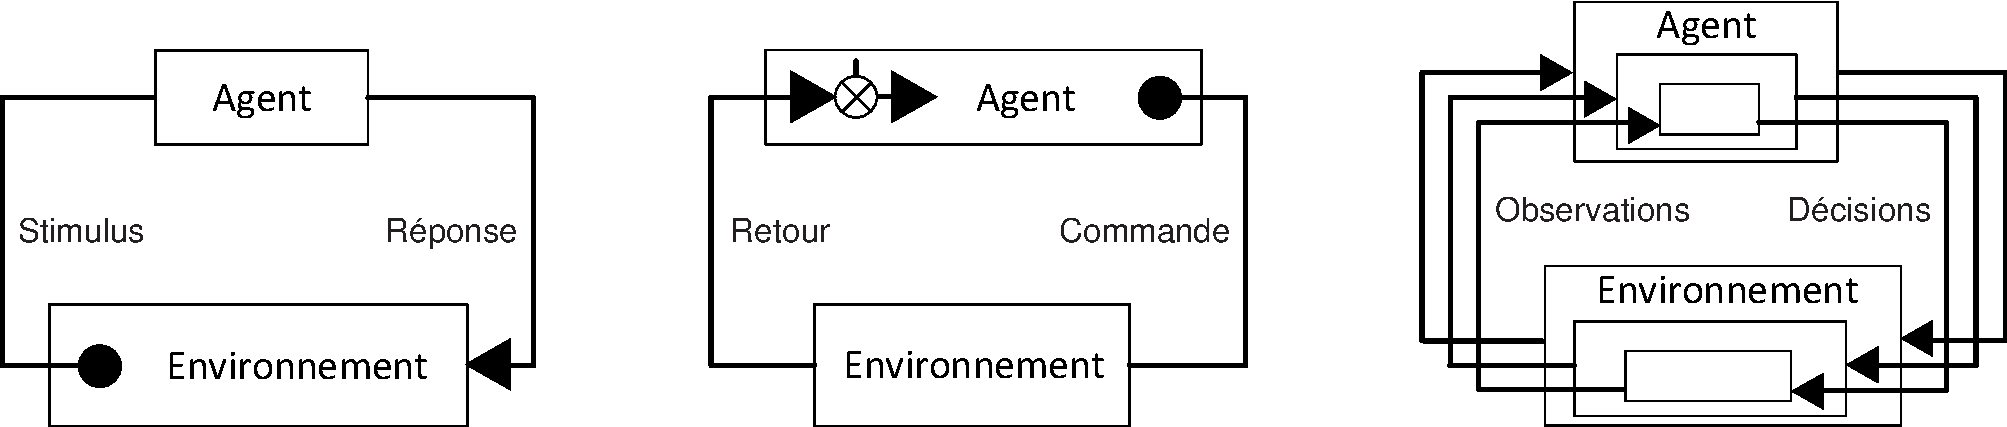
\includegraphics[width=0.9\textwidth]{Figures/1_dds2.pdf}
	\caption{Différentes déclinaisons du système de décision discret (DDS) dans lesquelles le début du cycle est matérialisé par une puce.
		Gauche: cycle stimulus $\rightarrow $ réponse. 
		Centre: cycle d'asservissement utilisé en cybernétique. La croix cerclée représente une opération de comparaison entre le \an{feedback} reçu et celui attendu.
		Droite: plusieurs cycles de décisions hiérarchiques imbriquées.
	}
	\label{fig:dds2}
\end{figure}

En Figure \ref{fig:dds2}, le schéma de gauche illustre un cycle initié par l'environnement: celui-ci envoie une information à l'agent, puis l'agent envoie une réponse.
%La puce noire illustre le début conceptuel du cycle d'interaction.
Le schéma central représente un cycle initié par l'agent, lequel transmets une commande à l'environnement, puis reçoit un retour qu'il compare à une valeur de consigne, selon in principe d'asservissement réactif utilisé en cybernétique.
Les cycles du DDS se succédant indéfiniment, la position du début et de la fin du cycle pourrait sembler sans importance. 
La façon dont l'ingénieur conçoit le début et la fin du cycle peut pourtant changer radicalement la façon dont il conçoit le \an{software}. 


Le schéma de droite de la Figure \ref{fig:dds2} montre des cycles d'interactions hiérarchiques imbriqués au cours desquels l'agent prend des décisions impliquant différentes échelles de temps. 
Le DDS permet de modéliser un telle dynamique impliquant différentes échelles de temps, car certaines parties des entrées et des sorties peuvent être respectivement lues et écrites moins vite que d'autres. 
Cette possibilité pourrait apporter des éléments de réponse à la critique de Weinbaum et Veitas en permettant une évolution du couplage entre l'agent et l'environnement impliquant des interactions qui s'exécutent à des échelles de temps variables pas nécessairement prédéfinies par le concepteur. 

%Ce dernier cas soulève la question évoqué par Weinbaum et Veitas de savoir comment le couplage entre l'agent et l'environnement peut évoluer en impliquant des types d'interactions situés à des échelles de temps variables avec le temps. 


\subsection{Représentation bayésienne}

\noindent
La représentation basée sur les réseaux bayésien offre un modèle complémentaire au cycle de décision discret qui prend en compte la diversité des entrées et sorties ainsi que leur possible parallélisme.
%Dans cette représentation, le monde constitué de l'organisme et de son environnement est représenté par un réseau bayésien (\an{Bayesian Network}, BN). 

Les réseaux bayésiens, \an{Bayesian Network} (BN), parfois appelés \an{belief networks}, sont des graphes acycliques directs dont les n\oe uds représentent des variables aléatoires et les arcs des dépendances probabilistes entre ces variables. 
Ils servent à représenter des connaissances à propos d'un domaine incertain.
Il en existe de nombreuses spécialisations adaptées à différent types de problèmes, par exemple les chaines de Markov cachées et les filtres de Kalman \cite{ben-gal_bayesian_2008}.
%et les réseaux bayésiens. 


La Figure \ref{fig:bn} montre un réseau bayésien minimal contenant deux variables $S$ et $O$ liées par une relation de dépendance signifiant que la probabilité que la variable $O$ prenne une valeur particulière $o$ dépend de la valeur $s$ prise par la variable $S$. 
Cette dépendance conditionnelle est notée $P(O=o | S=s)$, ou, plus concisément, $P(O|S)$, et se lit \og probabilité de $O$ sachant $S$ \fg.
Dans cet exemple, $S$ est un \emph{parent} de $O$, et $O$ un \emph{enfant} de $S$.
La nature acyclique du graphe est cruciale pour garantir qu'aucun n\oe ud ne soit son propre ancêtre.


\begin{figure}[ht]
	\centering
	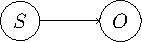
\includegraphics[width=0.2\textwidth]{Figures/2_bn.pdf}
	\caption{Réseau bayésien représentant que \og $S$ infulence son enfant $O$ \fg\ ou que \og $O$ dépend de son parent $S$ \fg\ avec la probabilité conditionnelle $P(O|S)$.
	%Les différentes probabilités impliquant ces deux variables sont liées par le théorème de Bayes: $P (O) P(S|O) = P(S)P(O|S) = P (O, S)$.
	}
	\label{fig:bn}
\end{figure}

Les variables dont les distributions de probabilité sont connues sont appelés des \an{evidences}. 
Le processus d'inférence bayésienne consiste à calculer les distributions de probabilité des autres variables qui leurs sont liées, pour possiblement obtenir la distribution de probabilité conjointe  (\an{Joint Probability Distribution}, JPD) de l'ensemble des variables du réseau.  

A titre d'illustration, $O$ peut représenter une observation acquise par un robot, et $S$ représente l'état de l'environnement caché au robot.
Le robot ne peut connaitre $S$ qu'indirectement par inférence à partir $O$.
Le réseau bayesien de la Figure \ref{fig:bn} formalise la relation de dépendance entre les deux.
Les distributions de probabilités associées à ces deux variables sont reliées par le théorème de Bayes donné en Equation \eqref{eq:bayes}. 

\begin{equation}
	\label{eq:bayes}
	P (O) P(S|O) = P(S)P(O|S) = P (O, S) 
\end{equation} 

%L'inférence bayésienne permet de calculer la dépendance probabiliste de l'état de l'environnement par rapport à l'observation, si les autres termes de l'équation sont connus. 
Imaginons que $O$ soit fournie par un capteur d'impact sujet à de fausses détections monté sur un bras robotique.
Le robot peut inférer la distribution de probabilités $P(S|O)$ qui représente les probabilités que l'environnement soit dans un certain état $s$ (i.e., objet présent) quand le robot acquiert une certain observation $o$ (i.e., impact).
Pour cela le robot doit connaitre la distribution de probabilités $P(O|S)$ que le capteur soit dans un certain état (i.e., impact) quand l'environnement est dans un certain état (i.e., objet). 
Il doit aussi connaitre les distributions de probabilités dites \emph{marginales}: $P(S)$ de chaque état possible de l'environnement, et $P(O)$ de chaque observation.


L'évolution des variables aléatoires au cours du temps peut être modélisée par un Réseau Bayésient Dynamique (\an{Dynamic Bayesian Network}, DBN) \cite{murphy_dynamic_2002}. 
Les DBNs sont des extensions des BNs définis par un réseau bayésien \an{prior}  $B_0$,  et un réseau bayésien \an{transition} $B_T$.
$B_0$ représente l'état initial des séries temporelles de variables, et $B_T$ leur transitions à chaque pas de temps.
Le nombre de pas de temps inclus dans $B_T$ définit la \emph{profondeur de la dépendance temporelle} du DBN, aussi appelée \an{Markov Window}.
Un $B_T$ avec deux tranches temporelles $t-1$ et $t$ est généralement suffisant car l'état de l'entité et de l'environnement au temps $t$ découle généralement de leur état au temps $t-1$ uniquement.
Cette hypothèse, dite \emph{markovienne d’ordre un}, est raisonnable dès lors que certaines variables encodent déjà des grandeurs intégratives, telles que des vitesses, des accumulations ou des traces mnésiques, assurant ainsi la prise en compte d’une histoire plus longue.

La partie gauche de la Figure \ref{fig:dbn} montre une représentation séquentielle d'un DBN du premier ordre.
La partie droite montre une représentation \emph{circulaire réduite} du DBN qui peut être utilisée si on n'a pas besoin de mettre en évidence la structure exacte de la dépendance temporelle. 


\begin{figure}[ht]
	\centering
	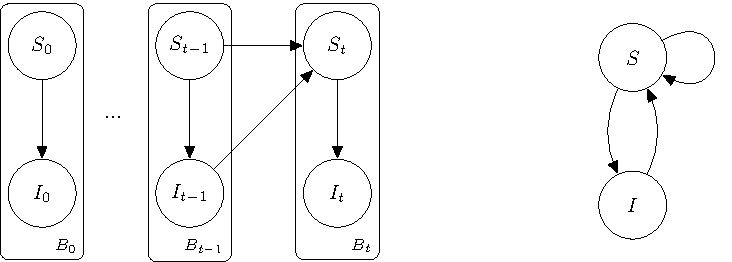
\includegraphics[width=0.6\textwidth]{Figures/2_dbn.pdf}
	\caption{Exemple de Réseau Bayésien Dynamique contenant deux séries de variables $S$ et $I$.
		Gauche: représentation séquentielle. 
    $B_0$ est le \an{prior}.
	$B_T$ est le graphe de transition de deux pas de temps.
	Droite: représentation circulaire réduite.}
	\label{fig:dbn}
\end{figure}

L'inférence bayésienne suppose de disposer, en amont, d'une modélisation des observations et des états possibles de l'environnement. 
En outre, lorsque le nombre de variables aléatoires et leurs cardinalités augmentent, le coût du calcul devient rapidement prohibitif. 
Il a été montré qu'il était\an{ NP-Hard} dans le cas général \cite{cooper_computational_1990}.
Pour ces raisons, nous ne pouvons pas l'utiliser directement en AI dévoppementale.

Sans mobiliser l'inférence bayésienne, je reconnais deux apports intéressants à la représentation par les réseaux bayésiens dynamiques. 
D'une part, elle permet de rendre compte de l'influence réciproque des différentes entrées et sorties au cours d'un même pas de temps.
Même si les DBNs sont cadencés en pas de temps discrets comme le DDS, ils offrent des possibilités de présentations plus complexes des interdépendances des entrées et des sorties. 
%sein d'un même réseau, ce qui offre un alternative au modèle d'alternance entre entrées et sorties. 
D'autre part, l'inférence bayésienne pose la question fondamentale d'inférer une connaissance du monde comme la meilleure hypothèse explicative (\an{best guess}) sur le monde que l'agent puisse formuler pour rendre compte la dynamique de ses interactions. 
Elle propose de réaliser cette inférence à partir d'observations qui ne constituent pas en elles-même une représentation directe de l'état du monde, que je qualifierai de \emph{signaux sensoriels non représentationnels}.



\subsection{Couverture de Markov}


\noindent
La dynamique d'une \emph{entité}, vivante ou non vivante, dans un environnement peut être représentée par un DBN dont un sous-ensemble $V_0$ des variables représente l'entité, et son complément $V_e$ représente l'environnement. 
L'ensemble $V_m$ des variables de $V_0$ qui ont des parents ou des enfants dans $V_e$ définissent l'interface entre l'entité et son environnement. 
Cet ensemble est appelé la  \emph{couverture de Markov} de l'entité. 


La couverture de Markov se scinde en deux sous-ensembles de variables selon que leurs relations de dépendance vont de l'intérieur vers l'extérieur ou l'inverse. 
Dans le cas d'un organisme vivant, l'ensemble $V_s \subset V_m$ des variables  qui sont influencés par les variables externes et qui influencent les variables internes sont les \emph{variables sensorielles} de l'organisme.
L'ensemble $V_a \subset V_m$ des variables qui sont infuencés par les variables internes et qui influencent les variables externes sont les \emph{variables motrices} de l'organisme. 
La Figure \ref{fig:blanket}, provenant de l'article de Alexander Ororbia et Karl Friston intitulé \og \an{Mortal Computation: A Foundation for Biomimetic Intelligence} \fg \cite[Fig.~5]{ororbia_mortal_2024} donne une représentation circulaire réduite de la couverture de Markov d'un organisme.

\begin{figure}[ht]
	\centering
	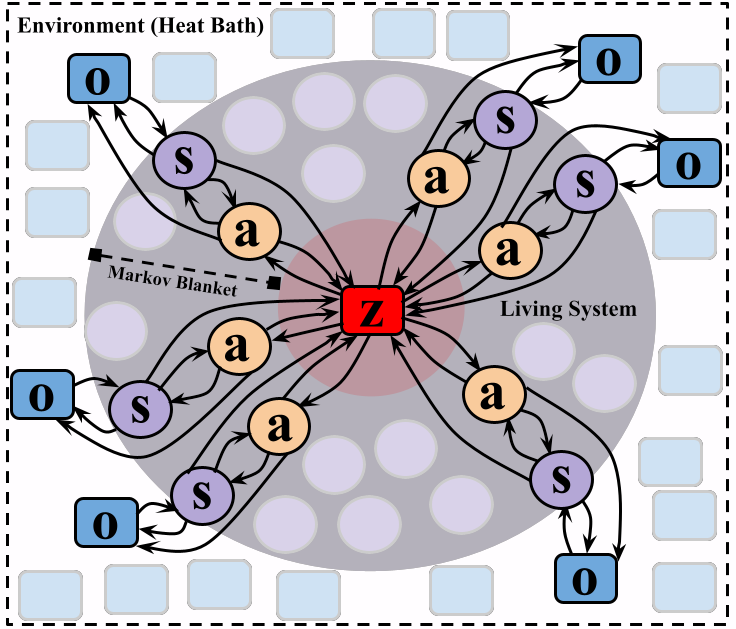
\includegraphics[width=0.4\textwidth]{Figures/1_blanket.png}
	\caption{Modélisation bayésienne d'un organisme dans son environnement \cite[Fig.~5]{ororbia_mortal_2024}.
		Z: état interne de l'organisme. 
		S: états des différents organes sensoriels.
		A: états des différents affecteurs.
		O: différentes variables représentant l'environnement.
		La distribution de probabilité de Z ne dépend que des noeuds S et A qui constituent la \emph{couverture de Markov} de l'organisme qui lui masquent les états des varibales $O$.}
	\label{fig:blanket}
\end{figure}


 


%En utilisant le théorème de Bayes, il est possible d'inféré les distributions de probabilité jointe des variables internes (\an{Joint Probability Distribution}, JPD) en fonction des distributions de probabilité des variables de la converture de Markov. 

%\begin{equation}
%	P(V)=\prod_{v\in V}P(v|pa(v))
%\end{equation}



Les théoriciens des réseaux bayésiens tels que Judea Pearl \cite{pearl_probabilistic_1988} ont montré que les statistiques des variables internes de l'orgnaisme sont entièrement définies par les statistiques des variables de la couverture de Markov, et donc indépendantes des statistiques des autres variables de l'environnement extérieur comme si le monde extérieur étaient caché par la couverture de Markov.
Ce résultat est employé en biologie pour signifier qu'il est mathématiquement impossible pour un organisme d'inférer la structure exacte du monde.
% car celle ci-est masquée par sa couverture de Markov.

Ce problème fondamental de l'inférence a été identifié sous de multiples formes. 
Legg \cite{legg_universal_2007} l'illustre par un exemple simple. 
Supposons que l'agent ait effectué la série d'observation \emph{2, 4, 6, 8}. 
Il pourrait inférer un modèle de l'environnement qui génère l'observation $o_t = 2t$. 
Ce modèle prédirait la prochaine observation au temps 5: $o_5 = 10$. 
Mais bien sûr, il existe une infinité de polynômes de degré $n$ compatibles avec une série de longueur $n$.
Par exemple, l'agent aurait aussi bien pu inférer le modèle  $o_t = 2t^4 - 20 t^3 + 70t^2 - 98t + 48$, compatible avec les 4 premières observations, mais qui prédirait une cinquième observation différente $o_5 = 58$.
Legg note que dans les tests psychotechniques, l'humain utilise naturellement le principe du rasoir d'Occam consistant à choisir le modèle le plus simple qui explique la série d'observations. 
Il propose que les systèmes d'intelligence artificielle devraient suivre le même principe.

Gary Drescher résume le problème de l'inférence ainsi: 
\begin{quote}
	\an{Whatever experiences an organism or mechanism has had, there are infinitely many mutually contradictory generalizations that are consistent with those experiences. Therefore, any induction apparatus must impose a choice among those consistent generalizations}
	\cite[p.~174]{drescher_made-up_1991}. 
\end{quote}

%Le fait même que les tests d'intelligence attentent que le sujet l'utilise indique que son utilisation efficace est considérée comme une facette importante de l'intelligence.   


Dans le cadre de l'IA développementale, les choix que nous imposerons à l'appareil d'inférence pourront être inspirés des connaissances-socle discutées en section \ref{sec:core}.



\subsection{Théorie de l'inférence active}
\label{sec:active_inference}


L'entité est comprise comme un \an{active observer} de son environnement qui agit et perçoit simultanément. 
La modélisation bayésienne voit la dynamique et l'auto-organisation de l'\an{observer} comme maintenant des croyances probabilistes représentées par les distributions de probabilité des variables de $V_0$ ($Z$, $S$, et $A$ en Figure \ref{fig:blanket}) à propos de l'\emph{observé} représenté par les distributions de probabilité des variables de l'environnement  ($O$ en Figure \ref{fig:blanket}).



Karl Friston et ses collorateurs ont proposé la vision que le \an{brain is an inference machine}. 

Le terme inference désigne le processus visant à tirer des conclusions sur l'état des variables d'un réseau sur la base de de connaissance préalables concernant d'autres variables. 
Plus précisément, l'inférence probabiliste consiste à calculer la distribution de probabilités de certaines variables connaissant la distribution de probabilité de variables données. 

La dynamique d'apprentissage de l'organisme est modélisée par un calcul bayésien qui converge vers une distribution de probabilité qui minimise les erreurs de prédiction que l'organisme fait à propos des variables de la couverture de Markov. 
Ce calcul d'inférence se fait de manière itérative en descendant un gradiant d'\emph{énergie libre} dans le réseau. 
L'état des variables internes de l'organisme $V_0$ représente finalement la meilleure hypothèse (\an{best guess}) que l'organisme peut faire à propos de l'état des variables cachées de l'environnement pour expliquer la dynamique de ses expériences d'interaction.






La théorie de l'inférence active (\an{Active Inference}) a été proposée par Karl Friston et ses collègues pour expliquer comment le cerveau inferre des connaissances sur le monde au cours de l'expérience interactive du sujet. 
Les états du système sensorimoteur entrainent des perturbations dans l'activité du cerveau qui infere des causes hypothétiques qui peuvent expliquer ces perturbations.


Le cerveau est compris comme en système en boucle fermée.
Les sens ne fournissent pas des données sur le monde en entrée du cerveau mais viennent simplement perturber cette boucle. 
Le processus de perception ne consiste pas à assembler des données reçues de sens mais consiste à inférer les causes dans le monde extérieur qui peuvent expliquer ces perturbations.

La théorie de l'inférence active propose que l'agent maintient deux modèles statistique: le \emph{generative model} et le \emph{recognition model}.
L'agent utilise le premier pour tenter de prédire les prochains signaux sensoriels qu'il va recevoir.
Il utilise le second pour inférer les causse hypothétiques qui peuvent expliquer les signaux sensoriels précédement reçus. 
Les deux modèles travaillent de concert: le modèle génératif utilise les convictions de l'agent au début du cycle d'interaction pour produire une estimation des futurs signaux sensoriels obtenus. 
Le modèle de reconnaissance récolte les signaux reçus pour mettre à jour les convictions sur l'état du monde extérieur.    

\begin{figure}[ht]
	\centering
	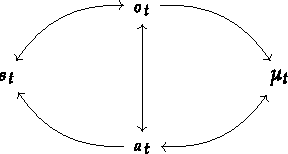
\includegraphics[width=0.4\textwidth]{Figures/2_active_inference.pdf}
	\caption{Représentation circulaire réduite du cycle l'inférence active d'après Albarracin et al. \cite[Fig.~1]{albarracin_sustainability_2024} montrant les influences mutuelles des  
	processus stochastiques au temps $t$: $o_t$ : signal sensoriel,
		$s_t$ : état de l'environnement, 
		$a_t$ : action de l'agent,
		$\mu_t$ : état interne de l'agent. 
	}
	\label{fig:inference_active}
\end{figure}

Mahault Albarracin, Maxwell Ramstead et leurs coauteurs proposent une présentation récente et épurée de la théorie de l'inférence active dans leur article \og \an{Sustainability under Active Inference} \fg\ \cite{albarracin_sustainability_2024}.
Un système qui contient un agent est modélisé par les quatre processus stochastiques, dont Figure \ref{fig:inference_active} offre une représentation circulaire réduite. 
Le processus $o$ est le signal sensoriel, $s$ l'état de l'environnement, $a$ l'action de l'agent, et $\mu$ : état interne (\an{beliefs}) de l'agent. 
Les flèches représentent les dépendances entre ces processus. 
Une différence importante avec le DDS de la Figure \ref{fig:dds} tient au fait que la majorité de ces influences sont bidirectionnelles au sein d'un même pas de temps $t$.
Au temps $t$, $o_t$ dépend de $s_t$ et de $a_t$ (le signal sensoriel dépend de l'état de l'environnement et de l'action),
$a_t$ dépend de $\mu_t$ et de $o_t$(les croyances internes et les signaux sensoriels influencent les actions),
$\mu_t$ dépend de $o_t$ et $a_t$ (les signaux sensoriels et les actions influencent les croyances internes),
et $s_t$ dépend de $a_t$ et de $o_t$ (l'environnement est affecté par l'action mais aussi par le signal sensoriel, selon le principe qu'une mesure peut modifier l'objet qu'elle mesure).
L'agent, au cours d'une période de temps allant de $0$ à un horizon temporel $T$ est défini par les processus $(o_t, a_t, \mu_t)_{t \in [0,T]}$.


La théorie de l'active inference a été elaborée à partir du concept du cerveau bayésien. 
C'est l'idée que notre cerveau raffine en parmanence un modèle interne du monde extérieur en agissant comme une machine d'inférence probabiliste. 
Le modèle génératif prédit en permanence l'état de l'environnement et compare ses prédictions avec les données des organes sensoriels. Quand un écart se produit, le cerveau met à jour son modèle.

La théorie de Active Inference est développée par une communauté autour de 
Karl Friston \cite{friston_active_2017} 

Ryan Smith, Karl Friston et Christopher White ont écrit un tutoriel \cite{smith_step-by-step_2022} pour utiliser cette théorie pour controler un agent dans un POMDP. 
L'idée est de guider les décisions de l'agent pour choisir les décisions qui apporteront le plus d'information à l'agent. 
Pour cela on utilise une mesure de l'information gagnée calculées selon le principe de l'énergie libre (free energy).
L'agent chosit la décision qui a le plus de chance de minimiser ses erreurs de prédiction futures. 

La théorie de l'inférence active rejette l'idée que les sens fourniraient directement une représentation de l'état de l'environnement au cerveau. 

Pierre-Yves Oudeyer remarque que les mathématiques d'inférence bayésienne nécessite que l'espace des états soit donné a priori.
De plus, il devient untractable quand l'espace d'états augmente \cite[e.g.]{buckley_free_2017}.:


\begin{quote}
	\an{Such a normative Bayesian framework requires that the modelled human subjects initially know the full space of possible hypotheses about possible world states, possible policies, possible model parameters, and possible model structures. [...] \\
		Active structured Bayesian inference is computationally very costly [Buckley et al., 2017], and quickly become computationally intractable for problems of moderate size }
	\cite[p.~9]{oudeyer_computational_2018}.
\end{quote}



\subsection{Inversion du cycle d'interaction}
\label{sec:inversion}

Un certain nombre d'auteurs ont fait remarquer que la direction du cycle d'interaction n'était pas neutre. 

La Figure \ref{fig:inversion} met matérialise le début et la fin du cycle d'interaction par une puce et un triangle noir. 
Le cycle inversé (à droite) offre deux avantages: 
\begin{itemize}
	\item il évite la références à l'action au cycle précédent $a_{t-1}$ : toutes les variables sont on cycle $t$.
	\item la récompense est une fonction de l'état $s_t$ obtenu après l'action, alors que dans le cycle classique la récompense (à gauche) est une fonction de l'état résultant de l'action précédente. 
\end{itemize}

On pourrait penser que puisque le cycle d'interaction se répète indéfiniment, peu importe quand il commence et quand il finit. 
Mais dans la pratique, la façon dont le designer comprend ce cycle influence la façon dont il conçoit l'agent.

\cite{georgeon_inverting_2014}

\begin{figure}[ht]
	\centering
	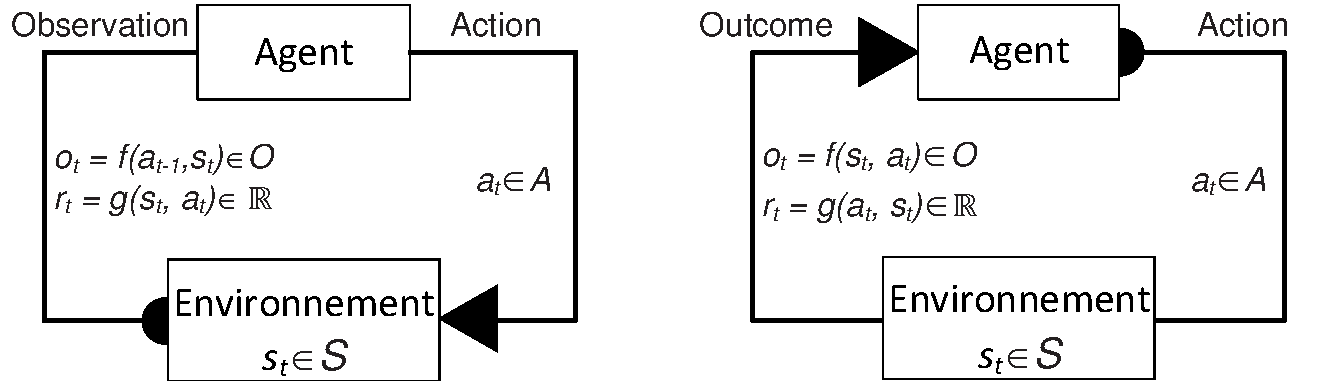
\includegraphics[width=0.8\textwidth]{Figures/3_inversion.pdf}
	\caption{L'inversion du cycle d'interaction \cite{georgeon_inverting_2014} montrant le début (puce noire) et fin (triangle noir) du cycle.
		Gauche: cycle des POMDP classiques.
		Droite: cycle inversé.}
	\label{fig:inversion}
\end{figure}




\subsection{Finalité et motivations de l'agent}
\label{sec:motivation_intrinseque}

\noindent
La distinction entre motivation extrinsèque et motivation intrinsèque est relativement intuitive quand on parle des motivations humaines: on fait quelque chose soit pour obtenir un certain résultats final (motivation extrinsèque) soit pour la satisfaction de le faire (motivation intrinsèque).
La distinction "telique" / "atelique" est utile pour distinguer les deux types d'activités. 
Une activité qui est faite par motivation extrinsèque est dite "télique", une activité qui est faite par motivation extrinsèque est dite "atélique". 

Cependant cette distinction devient plus délicate à définir dans le cas d'un système artificiel.
Le terme même de "motivation" est un terme qui relève de la psychologie, c'est pourquoi le qualificatif "télique" "atélique" appliqué à la tache est plus utile. 

L'article de Pierre-Yves Oudeyer compte parmi les premiers qui ont placé ce terme dans le domaine de la robotique  \cite{oudeyer_intrinsic_2007}.
\og \an{What is intrinsic motivation? A typology of computational approaches} \fg \cite{oudeyer_what_2007} 

Un programme qui joue aux échec est un bon exemple de système artificiel "dirigé par une motivation extrinsèque". 
On peut créer un programme qui apprend à jouer au échecs en lui donnant une récompense positive quand il gagne et négative quand il perd, et nulle quand il fait un match nul. 
C'est un cas emblématique d'apprentissage par renforcement en situation markovienne.
Pour cela il faut implémenter un environnement qui soit capable de détecter les situations gagnantes, perdantes, et nulles sur l'échiquier de façon à générer ce signal d'erreur. 
Examinons cela plus en détail.
On pourrait implémenter un système "arbitre" complètement extérieur au programme de jeu qui déclarerait la fin de partie. 
Cet arbitre doit intégrer toutes les règles du jeu pour déterminer si l'un des deux rois est en situation d'échec et mat. 
Il doit aussi surveiller les cas de figures qui mènent à une situation de match nul par différentes modalités (pat, etc.) ce qui n'est pas immédiat dans le cas de nul par répétition de position. 
En pratique il n'est pas nécessaire d'implémenter un arbitre. 
Notons que le programme lui même doit pouvoir détecter la fin de partie et son status.
Il n'est donc pas nécessaire d'implémenter un arbitre externe, on peut utiliser la capacité du programme lui meme pour connaitre le gagnant et générer le signal de récompense. 
Mais si le signal de récompense est interne au programme, ne peut on pas dire que la récompense est intrinsèque. 


Il est plus simple d'implémenter quelques sous-programme dédiés à la détection 

Mais ce qui se passe en pratique c'est que c'est le programme lui meme qui évalue la situation et qui génère la récom 

Ron Sun s'est posé la question d'intégrer des principes motivationnels dans une architecture cognitive \cite{sun_motivational_2009}.


Il serait peut etre plus judicieux de distinguer entre "objectifs internes" et "objectifs externes".
La notion de motivation extrinsèque pose problème car toute motivation peut etre considérée comme intrinsèque. 
La notion de motivation intrinsèque doit deux plutot etre compris comme n'antinomique de "récompense externe". 

\subsection{Curiosité artificielle}
\label{sec:curiosite}

Dans son livre \an{The new science of curiosity}, le roboticien Goren Gordon passe en revue différentes approches pour créer des agents artificiels intelligent et mieux comprendre la curiosité chez l'humain et l'animal \cite{gordon_new_2018}. 

Pierre-Yves Oudeyer fait la distinction entre les approches normatives et les approches heuristiques pour générer un comportement de curisité \cite{oudeyer_computational_2018}.
Les approches normatives utilisent des algorithms de maximization d'une fonction d'utilité basée sur le gain d'information ou la réduction d'incertitude, inspirée de la théorie de l'information et de l'inférence bayésienne.
A l'opposé, Les approches heuristiques tentent d'évaluer des zones locales offrant des potientiels d'apprentissage. 
Une des heuristiques proposées est basée sur la \an{learning progress hypthesis} qui consiste à orienter le robot vers les zones ou l'erreur de prédiction diminue de manière mesurable en évitant les zones trop faciles ou trop difficiles pour organiser le curriculum d'exploration.
Un autre exemple est Le processus d'exploration de buts intrinsèquement motivés (GEP-PG) qui découple exploration et exploitation via des populations de trajectoires. 
Cette heuristique a été  implémentés pour l'apprentissage de la locomotion et de la manipulation d'objets souples dans une étude intitulée \an{Intrinsically motivated goal exploration processes with automatic curriculum learning} \cite{forestier_intrinsically_2022}. 

Oudeyer note que les approches normatives et heuristiques ne sont pas antagonistes. 
Il se pourrait que les approches normatives permettent de diriger l'attention sur des opportunités d'apprentissage existant dans des échelles de temps courtes, mais que pour des opportunités d'apprentissage à plus longue échelle de temps, les heuristiques soient plus utile pour choisir des activités comme les jeux ou des défis. 

\subsection{Mesure de l'information gagnée}

\noindent
Dans la théorie de l'information de Claude Shannon, l'information qu'un agent possède à propos d'une variable $X$, pouvant prendre $n$ valeurs distinctes, est représentée par une distribution de probabilités $d= (p(x_1), p(x_2), ... , \allowbreak p(x_n))$.
Cette distribution, parfois appelée \an{belief state}, signifie que l'agent \og croit \fg que, pour chacune valeurs $x_i$ parmi les $n$ valeurs possibles de $X$, il y a une probabilité $p(x_i)$ que $X$ soit égale à $x_i$. 

Shannon interprète la grandeur $I(x_i) = -log_2(p(x_i))$ comme la quantité d'information (exprimée en nombre de bits) apportée par la connaissance que $X = x_i$. 
Intuitivement, quand l'agent reçoit une valeur qu'il attendait, il gagne peu d'information, mais quand il reçoit une valeur qu'il jugeait improbable, il en gagne beaucoup.
$I(x_i)$ peut aussi s'interpréter comme la \og surprise attendue \fg  par l'agent. 
Plus $x_i$ est probable ($p(x_i)$ proche de 1), plus l'agent s'attend à une surprise faible ($I(x_i)$ proche de 0) s'il observe $X = x_i$. 
A l'inverse, quand $p(x_i)$ approche 0, la surprise attendue pour l'observation de $X=x_i$ tend vers l'infini. 
Sur cette base, Shannon définit l'entropie de $d$ comme l'espérance de surprise (\an{expected surprise}), obtenue en pondérant chaque valeur de surprise par sa probabilité d'occurence.
L'entropie $H(d)$ est donc formalisée par l'Equation \eqref{eq:shannon} dans laquelle l'indice $i$ est omis pour simplifier :

\begin{equation}\label{eq:shannon}
	H(d) = - \sum_{p(x) \in d} p(x) log_2(p(x))
\end{equation}

Lorsque la probabilité $p(x_i)$ d'une valeur $x_i$ tend vers 1 tandis que celles des autres valeurs tendent vers 0, $H(d)$ tend vers 0.
Un \an{belief state} d'entropie nulle correspond donc à une situation dans laquelle l'agent \og se sent certain \fg de la valeur de $X$. 
Inversement, lorsque toutes les valeurs possibles sont équiprobables ($p(x_i) = 1/n$ pour tout $i$), l'entropie atteint sa valeur maximale qui vaut $H(d) = log(n)$. 
Un \an{belief state} d'entropie maximale traduit le fait que l'agent estime n'avoir aucune information sur $X$.
L'entropie du \an{belief state} ne fournit donc pas d'indication sur la justesse objective de la croyance de l'agent.
Elle doit plutôt être interprétée comme une mesure de son degré de certitude subjective : elle quantifie à quel point l’agent se considère sûr de sa propre croyance, qu’elle soit juste ou fausse.

Dans le cas d'un agent interagissant avec son environnement de manière cyclique, et pour lequel la variable $X$ représente le signal sensoriel reçu au cycle $t$, on peut implémenter une distribution $d_t$ pour représenter les probabilités estimées par l'agent du prochain signal sensoriel. 
Dans ce cas, la baisse de l'entropie de $d$ au cours du temps peut être interprétée comme un indicateur des progrès d'apprentissage de l'agent. 

% On peut également calculer une fonction de perte (\an{loss}) 

\subsection{Principe d'énergie libre}

Il existe différentes mesures refléter l'évolution du \an{belief state} de l'agent. 
L'une d'elle est la divergence de Kullback-Leibler



\subsection{Autonomie constitutive}



\subsection{Théorie de l'enaction}
\label{sec:enaction}

La théorie de l'enaction provient tu terme anglais \an{to enact} qui signifie mettre en action ou mettre en œuvre. 
Francisco Varella et humberto Maturana \cite{varela_embodied_1993} sont à l'origine de la théorie de l'enaction.

Selon Hutto et Myin \cite{hutto_radicalizing_2013}, la théorie de l'enaction peut être divisée en trois courants majeurs: \emph{autopoietique}, \emph{sensorimoteur} et \emph{radical}. 
Le courant autopoiétique \cite{varela_embodied_1993} s'intéresse à fonder la cognition sur les processus biologiques des systèmes vivants. 
Le courant sensorimoteur \cite{oregan_sensorimotor_2001} s'intéresse à expliquer l'expérience perceptive par la maitrise de contingence sensorimotrices. 
Le courant radical \cite{hutto_radicalizing_2013} porte son attention sur la nature anti-représentationnelle de l'enactivisme. 
 

Tom froese et Tom Ziemke ont propose l'IA enactive. 
\cite{froese_enactive_2009}

Weinbaum note que le concept de \an{operational closure} est un concept central de la théorie de l'enaction \cite{weinbaum_open_2015}: 

\begin{quote}
\an{An identity is generated whenever a precarious network of dynamical processes becomes operationally closed. A system is operationally closed if, for any given process P that forms part of the system (1) we can find among its enabling conditions other processes that make up the system, and (2) we can find other processes in the system that depend on P . This means that at some level of description, the conditions that sustain any given process in such a network always include those conditions provided by the operation of the other processes in the network, and that the result of their global activity is an identifiable unity in the same domain or level of description (it does not, of course, mean that the system is isolated from interactions with the environment). Autonomy as operational closure is intended to describe self-generated identities at many possible levels} (Di Paolo, Rohde, and De Jaegher, 2010, p. 38).
\end{quote}

Weinbaum ajoute le concept de \an{fluid identity} comme une \og \an{modification of the enactive approach to cognition based on replacing individuals with individuation} \fg.

De plus, dans la théorie de l'enaction, la valeur n'est pas données: \\
\begin{quote}
	\an{Though we accept that values are intrinsic to sense-making, we do not agree that values must precede any intelligent activity or sense-making in order to guide them; nor that they are necessarily preceded by the establishment of an autonomous identity. Rather, values are products of an ongoing individuation. Emerging values in the process
	of individuation carry their own problematic as they are initially non-coherent or even conflicting } \cite[p.~28]{weinbaum_open_2015}.
\end{quote}

Identity is nothing more than a set of variables being kept within a certain range of values. Identity and values therefore co-define each other.


\subsection{Théorie des contingences sensorimotrices}
\label{sec:SMC}

\noindent
Kevin O'Regan et Alva Noë ont proposé la \emph{Théorie des Contingences Sensorimotrices} \cite{oregan_sensorimotor_2001}.
Ils expliquent cette théorie en utilisant la métaphore d'une équipe d'ingénieurs qui télé-comman\-derait un sous-marin comme illustré en Figure \ref{fig:smc}. 
Un monstre marin aurait mélangé toutes les connexions à destination et en provenance des différents éléments du sous-marin: caméras, sonars, bras robotique, actionneurs, capteurs. 
Ce qui apparait sur les écrans et les voyants n'a plus aucun sens. Les commandent n'ont plus leurs fonctions habituelles. 

\begin{figure}[ht]
	\centering
	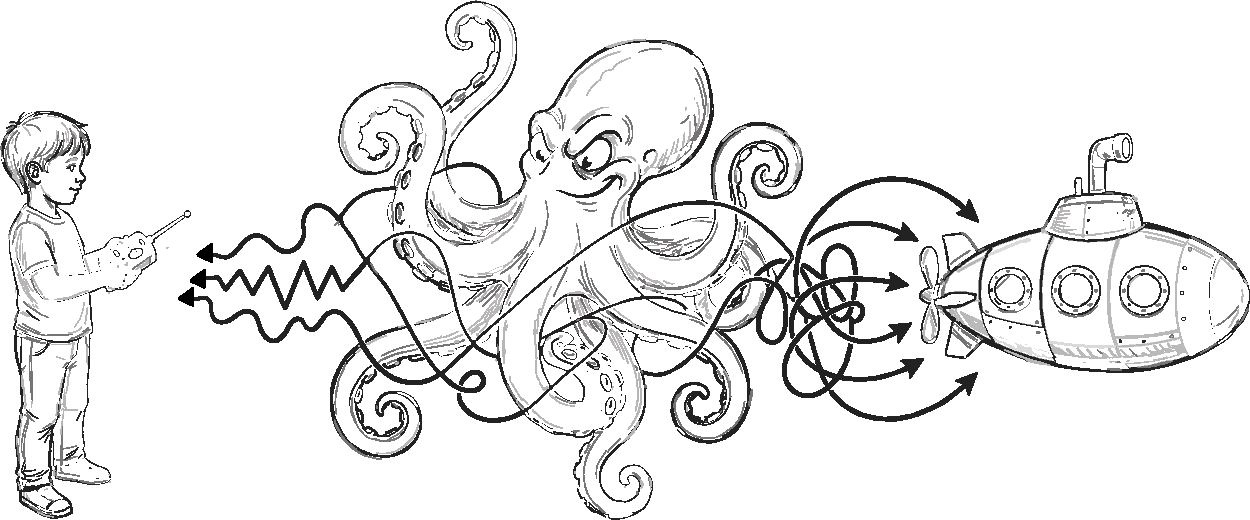
\includegraphics[width=0.8\textwidth]{Figures/2_smc.pdf}
	\caption{Métaphore du sous-marin de O'Regan et Noë \cite{oregan_sensorimotor_2001}.
		Le cerveau serait dans la situation de la personne qui télécommande un sous-marin (qu'il ne voit pas), alors que toutes les connexions entrantes et sortantes ont été mélangées par un monstre marin. 
	}
	\label{fig:smc}
\end{figure}

En observant la \emph{structure des changements} qui se produisent quand ils appuient sur les boutons, les ingénieurs devraient pouvoir comprendre ce que les commandent et les voyants signifient. Selon O'Regan et Noë : 

\begin{quote}
%\an{Imagine a team of engineers operating a remote-controlled underwater vessel exploring the remains of the Titanic, and imagine a villainous aquatic monster that has interfered with the control cable by mixing up the connections to and from the underwater cameras, sonar equipment, robot arms, actuators, and sensors. What appears on the many screens, lights, and dials, no longer makes any sense, and the actuators no longer have their usual functions. What can the engineers do to save the situation? By observing the \emph{structure of the changes} on the control panel that occur when they press various buttons and levers, the engineers should be able to deduce which buttons control which kind of motion of the vehicle, and which lights correspond to information deriving from the sensors mounted outside the vessel, which indicators correspond to sensors on the vessel’s tentacles, and so on.}
\an{There is an analogy to be drawn between this example and the situation faced by the brain. From the point of view of the brain, there is nothing that in itself differentiates nervous influx coming from retinal, haptic, proprioceptive, olfactory, and other senses, and there is nothing to discriminate motor neurons that are connected to extraocular muscles, skeletal muscles, or any other structures.}
\cite{oregan_sensorimotor_2001}
\end{quote}


Puisqu'il n'y a pas de distinction à priori entre les différents signaux sensoriels et moteurs, O'Regan propose que ce qui distingue les différentes expériences perceptives soit les lois qui gouvernent la \emph{structure des contingences sensorimotrices}. 
Selon lui, l'expérience de \emph{percevoir} se produit quand l'organisme maitrise ces lois.

Cette conception rappelle la phrase de Merleau-Ponty citée en Section \ref{sec:phenomenologie}: \og la vision est le palpé de l’œil \fg. 
En maintenant vivante cette conception phénoménologique de la perception à l'ère de l'informatique,  O'Regan aide à imaginer comment elle pourrait être implémentée dans un système artificiel. 
Dans ce nouveau contexte, les contingences sensorimotrices correspondent à la dynamique des signaux moteurs et sensoriels émis et reçus par un système informatique ou robotique. 

O'Regan ne se prononce pas sur la manière dont les signaux moteurs et sensoriels sont constitués, mais, dans un commentaire ouvert à son article, Donald Laming  insiste sur l'importance de distinguer entre \emph{contingences sensorimotrice} et \emph{contingences motosensorielles} \cite{laming_distinction_2001}. 
Selon Laming, ces deux  types de contingences sont radicalement différentes. 
Le terme \an{sensorimotor} suggère le point de vue d'un observateur tiers pour qui le \an{sensor} constituerait la variable indépendante, et le \an{motor} la variable dépendante. 
En revanche, pour le sujet lui même, le \an{motor} constitue la variable indépendante et le \an{sensor} la variable dépendante. 
Entre les deux cas, les dynamiques des statistiques sont radicalement différentes. 
Laming propose donc le terme \an{motorsensory contingencies} pour rendre compte du point de vue subjectif du sujet percevant. 


\subsection{L'émergence de sémantique ancrée dans l'expérience sensorimotrice}

Tous les modèles sont "ancrés" dans quelque chose. 
Par exemple les LLMs sont ancrés dans leurs données d'entrainement. 
La question est de savoir quel sorte d'ancrage on veut. 
A quoi est ancré la connaissance ? Est elle ancrée dans le langage, dans la physique ? dans l'expérience 
? % Dr Jeff Beck machine learning street talk


Pei Wang \cite{wang_experience-grounded_2005} pose la question de l'émergence sémantique ancrée dans l'expérience sensorimotrice (\an{experience-grounded semantics}).
A la différence des raisonnements mathématiques fondés sur des axiomes, l'architecture NARS (\an{Non Axiomatic Raisoning System}) effectue un raisonnement non axiomatique, basés sur l'expérience.

Récement, Bowen Xu \cite{xu_brain-inspired_2025} a utilisé ce principe pour implémenter un système d'apprentissage séquentiel. 
Il soulève la question de l'interpretabilité du modèle: 
\begin{quote}
	Explainability is a crucial issue in AI safety, and a major criticism of neural networks is their lack of transparency: these models often operate as black or grey boxes, making it difficult for developers to understand their internal workings and address unexpected behaviors. One approach to addressing this issue is to ensure that a model adheres to a logical framework. In other words, a model is considered interpretable if it can be described through logical representation \cite[p.~1]{xu_brain-inspired_2025}.
\end{quote}


Citer aussi "Behavior Is Everything: Towards Representing Concepts with Sensorimotor Contingencies" de Dileep George et al.


\subsection{Modèle du monde}

David Ha et Jürgen Schmidhuber ont proposé un système capable d'apprendre un modèle du monde dans des environnement d'apprentissage par renforcement populaires \cite{ha_world_2018}.

Karl Friston et ses coauteurs abordent la question de l'apprentissage d'un \an{world model} dirigé par le principe d'énergie libre \cite{friston_world_2021}

Yann LeCun a argumenté que le chemin vers IA de niveau humain dans la prochaine décennie reposera sur des modèles du monde qui permettent le raisonnement et la planification.
\og \an{Joint-Embedding Predictive Architecture} \fg (JEPA) \cite{balestriero_lejepa_2025}


\subsection{Apprentissage et monde \og ouvert \fg}

Le monde physique nous semble offrir une infinité de futurs possibles qui peuvent se dérouler sur des trajectoires éternellement changeantes. 
Pour cette raison, nous le qualifions \og d'ouvert \fg dans le sens ou l'espace des possibles n'est pas délimité.
Par contraste, nous qualifions certains environnements de \og fermés \fg quand leurs trajectoires futures nous apparaissent contrainte par leur dynamique interne. 
Les jeux de plateau comme le jeu d'échec constituent un exemple emblématique. 
Ils sont contraint par un ensemble bien défini de règles qui spécifient leurs états et transitions possibles, ainsi que l'objectif à atteindre. 
La distinction n'est pourtant pas toujours évidente à définir. 
Qu'en est il par exemple d'un jeu de billard ? 
Il semble qu'on puisse qualifier le jeu de billard d'environnement fermé si on néglige les influences externes à la table, telles que les vibrations provenant du sol, les déplacement de l'air, etc. 
Dans ce cas un environnement \og continu \fg (par opposition à \og discret \fg dans le sens ou les boules peuvent occuper une infinité d'états possibles ) peut être considéré comme un environnement fermé mais uniquement en tant que représentation théorique qui considère les influences extérieures comme négligeables. 
Il faut toutefois noter que du point de vue d'un jour, que ce soit sur un terrain discret comme les échecs, ou continu comme le billard, bien que le terrain soit un terrain fermé, le déroulement futur de la partie est influencé par une cause externe qui est le joueur adverse. 
Cependant, si on fait l'hypothèse que le joueur adverse joue dans le but de gagner le jeu, on peut modéliser son processus de décision de manière identique à celui du système d'IA lui même. 

En général la recherche en IA vise à construire des systèmes capables de prendre une décision optimum la base d'une représentation de l'environnement et de sa dynamiques (le \an{problem space}) en intégrant éventuellement un facteur d'inconnu sous la forme d'un processus aléatoire. 
Beaucoup de recherches en IA se consistent à rechercher la décision optimum dans un environnement modélisé dans le système d'IA. 
Le système d'IA effectue des prédictions sur la base d'un monde fermé, le \an{problem space}.
Cette décision peut etre mise en oeuvre dans le monde physique, et elle sera appropriée si le modèle de monde utilisé par l'IA est suffisamment fidèle à la réalité pour .  

L'étude de l'adaptation de l'IA à des environnements physiques complexes devient de plus en plus un sujet d'attention au fur et à mesure que les applications de l'IA se développent, comme en témoigne la publication récente d'un numéro spécial de le revue \an{Artificial Intelligence}  intitulée \an{Open-world AI} \cite{holder_introduction_2025}, ou la création d'un nouveau \an{Workshop on open-world agents} à la conférence NeurIPS 2024. 
La question de définir un environnement de test qui soit ouvert se pose alors. 
Elle peut prendre des formes très variées selon qu'on se place dans le domaine des ontologies, de la vision artificielle, ou des l'apprentissage par renforcement. 
On peut se référer à la construction incrémentale d'ontologies, la catégorisation d'images non supervisée \cite{jafarzadeh_review_2022} ou à une étude d'apprentissage par renforcement \an{open-ended} \cite{team_open-ended_2021}. 


Dans son article \an{What Do You Mean by ``Open Worl''?}, Bowen Xu note que la notion de monde ouvert implique deux choses: 

1. Les expériences passées de l'agent ne sont pas toujours directement applicables à une situation nouvelle, 
\begin{quote}
	Whether we assume that the laws governing the world are unchanging but beyond the machine’s reach, or that no such unchanging laws exist, the implication for AI remains the same: intelligent machines must be theoretically prepared for these potential changes, rather than relying on the assumption that the world’s rules are fixed and pre-programmed by human developers \cite[p.~3]{xu_what_2024}.
\end{quote}

2. La tache de l'agent ne soit pas prédéfinie par le concepteur:  
\begin{quote}
	In fully open worlds, tasks are not predefined by human developers, so researchers must focus on problem-independent aspects of intelligence 
	\cite[p.~3]{xu_what_2024}.
\end{quote}
Il argumente que tester l'existence d'environnements de test ouvert pourra générer de nouveaux problemes d'apprentissage en IA. 


Pour moi, ce qui est important de souligner c'est que ce n'est pas une propriété absolue du monde en soi mais une propriété relative selon que le monde apparait ouvert par par rapport au système qu'on considère. 

C'est un système dont le designer ne connait pas a priori le nombre d'états, rendant inapplicable les algorithmes qui préssuposent l'espace d'états (state space). 
Compte tenu du fait qu'un système de décision artificiel base ses prédictions sur son modèle de monde interne qui est nécessairerment fermé, la recherche pour permettre à des systèmes artificiels de démontrer une intelligence en monde ouvert doit porter sur la capacité du système à faire évoluer son modèle du monde à partir de ses expériences effectuées dans le monde ouvert. 
Notons le state space peut etre infini et pour autant fermé. 
ON passe généralement d'une mathématique en monde fini à une mathématique en monde conitnu en changeant les sommes en intégrales et en raisonnant sur des distributions de probabilités. 




\subsection{L'apprentissage des structures spatiales}

\noindent
La question de savoir si l'espace physique est constitue un \og a priori de l'entendement \fg comme Kant l'a suggéré ou s'il est un concept construit à partir de l'expérience sensorimotrice est encore d'actualité dans les recherches en intelligence artificielle. 
On trouve souvent attribuée au mathématicien Henri Pointcaré la paternité de l'idée que la connaissance de l'espace pourrait etre construit à partir de l'expérience sensorimotrice: 

\begin{quote}
\og Localiser un objet, c'est représenter les mouvements que l'on devrait exécuter pour l'atteindre. 
Il ne s’agit pas de représenter ces mouvements dans l’espace, mais de se représenter seulement les sensations musculaires qui accompagnent ces mouvements et qui, elles, ne supposent pas l’existence de l’espace. \fg \cite[p.~67]{pointcare_science_1902}.
\end{quote}

Pointcaré a suggéré que le concept d'espace émergait à travers la découverte de changement sensoriels compensables qui sont générés par un changement dans l'environnement mais qui peuvent être annulés par un action de l'agent. 

Bowen Xu et Pei Wang \cite{xu_essence_2025} expriment l'intérêt de ce genre de recherche : 
\begin{quote}
\an{While the 3D assumption may suffice for practical purposes regarding the physical world, we argue that dropping it has theoretical significance. 
	AGI research aims not only to engineer machines but also to uncover principles of intelligence. 
	Different studies strike a balance between these two objectives. 
	Understanding how spatial sense emerges, without assuming space, advances the latter goal, since we can imagine a system without any notion of the physical space in the beginning but capable of learning to interact with the physical world and developing spatial sense} \cite[p.~2]{xu_essence_2025}
\end{quote}

Simon Gay s'est intéressé à ce sujet dans sa thèse de doctorat \cite{gay_autonomous_2017} 

Citons l'article d'Alban Laflaquière et Michael Garcia Ortiz \og \an{Unsupervised Emergence of Egocentric Spatial Structure from Sensorimotor Prediction} \fg \cite{laflaquiere_unsupervised_2019}.
Alexander Terekov et Kevin O'Regan ont proposé un modèle d'apprentissage de l'espace à partir des contingences sensorimotrices \cite{terekhov_learning_2019},  utilisant la question de l'émergence de structures spatiales comme un exemple de l'émergence de concepts abstraits
Les travaux récents de l'équipe de Deleep George font peut être partie des plus avancées sur cette question à ce jour \cite{raju_space_2022}.

Ces travaux ont en commun le fait que l'apprentissage des structures spatiales est démontrée dans un environnement fermé à la complexité limitée. 
A notre connaissance, il n'existe pas de travaux démontrant l'apprentissage de structures spatiales en environnement ouvert. 



\section{Conclusion}

L'inversion du cycle d'interaction considère le signal sensoriel comme un feedback de l'action et non comme un percept.


L'apprentissage sur différentes échelles de temps est un problème souvent identifié mais qui reste encore ouvert 
(voir les références dans l'article ECA)

Le stade de la maitrise de l'appareil sensorioteur, le premier stade identifié par Piaget, n'est pas encore résolu en intelligence artificielle. Pourtant il s'agit bien d'un problème qui relève de l'intelligence au plein sens du terme. Citer Josha Back, fondateur de Californian Institute of Machine Consciousness.